\documentclass{beamer}
\mode<presentation>
%==================  필요한 패키지 설정 ===============
\usepackage{verbatim}
\usepackage{pdfpages}
\usepackage{multimedia}
\usepackage{animate}
% 
\usepackage{bm}% bold math
\usepackage{amsmath,amssymb,amscd}
\usepackage{subeqnarray}
\usepackage{mathptmx}
% 
\usepackage{helvet}
\usepackage{courier}
\usepackage{relsize}
% 
\usepackage{colortbl}
\usepackage{wasysym}
%
\usepackage{tikz}
\usetikzlibrary{arrows,shapes,calc,patterns}
\tikzstyle{every picture}+=[remember picture]
\usetikzlibrary{%
	decorations.pathreplacing,%
	decorations.pathmorphing%
}
% ================== 한글 사용 =====================
\usepackage{dhucs}
\usepackage{ifpdf}
\ifpdf
%\input glyphtounicode\pdfgentounicode=1
\fi
%==============================================
\setbeamertemplate{footline}[frame number]
%\usepackage{default}

%==================  표지 만들기 =====================
\title % (optional, use only with long paper titles)
{두번째: SAM}
%\subtitle{\LaTeX 기초강좌 (2008년 가을, 공주대학교)}


\author{강성원}													% 저자(발표자)

% Till Tantau\author{{1} \and
% J\"{o}rg Cassens\inst{2}

\institute[KEI] 															% (optional, but mostly needed) 소속기관 약자 표기
{KEI}													% 표지에 나타나는 소속기관 full name
% - Use the \inst command only if there are several affiliations.
% - Keep it simple, no one is interested in your street address.

\date[08-11-09] 														% (optional, should be abbreviation of conference name)
{2016.08.04}																			% 날짜 지정: \today
% - Either use conference name or its abbreviation.
% - Not really informative to the audience, more for people (including
%   yourself) who are reading the slides online

\subject{Beamer}

% ====================  차 례 ======================
\AtBeginSection[]
{
	\begin{frame}<beamer>
		\frametitle{차 례}
		%\tableofcontents
		\tableofcontents[currentsection]
		%\tableofcontents[currentsection,currentsubsection]
	\end{frame}
}
\AtBeginSubsection[]
{
	\begin{frame}<beamer>
		\frametitle{차 례}
		%\tableofcontents
		%\tableofcontents[currentsection]
		\tableofcontents[currentsection,currentsubsection]
	\end{frame}
}

%===============================================

\begin{document}
%=================  표지를  화면으로 나타나기 =============
\begin{frame}
	\titlepage
\end{frame}
%===============================================
%
\begin{frame}{개관}
	\tableofcontents
\end{frame}
%--------------------------------------------------
\section{SAM 구축 순서}
%===============================================
%------------------------------------------------------------------------------
\begin{frame}{순서}
	\begin{enumerate}
		\item {산업 mapping 확정}
		\item {IO aggregation}
	    \item {SAM 구축 }
		\item {set 점검}
	\end{enumerate}
\end{frame}
%------------------------------------------------------------------------------

\section{1. 산업 mapping}
%------------------------------------------------------------------------------
\begin{frame}
	\frametitle{1. 산업 mapping 확정}
	384개 기본부문 $\rightarrow$ 37개 산업 (표준모형) $\rightarrow$ 7개 산업 (Prototype)\
	(indcode\_20161202.xlsx, indcode\_20161202.csv)
	\begin{figure}
		\centering
		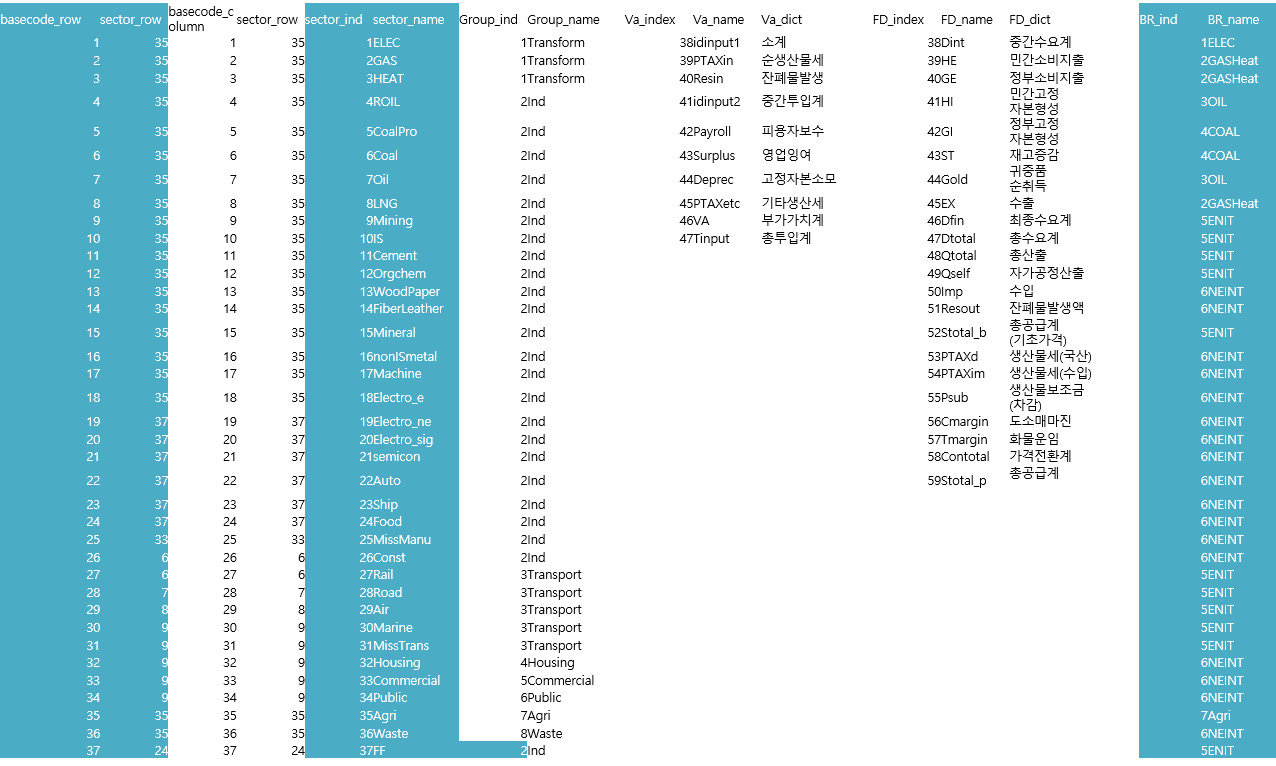
\includegraphics[width=1.00\textwidth]{map.png}
	\end{figure}
\end{frame}
%------------------------------------------------------------------------------

\section{ 2. IO aggregation}
%------------------------------------------------------------------------------
\begin{frame}
	\frametitle{2. IO aggreation}
	IO aggregation : 차원을 줄인 IO 만들기 (agg\_1202.r, agg\_ghg\_1202.r)
		\begin{itemize}
		\item {agg\_1202.r : IO 차원 줄이기}
			\begin{description}
				\item[input]{IOT\_b.csv (기초가격산업연관표), indcode\_20161202.csv (산업 mapping)}
				\item[output]{IO\_model\_1202.csv (37개 산업 IO), IO\_B\_1202.csv (7개 산업 IO)}
			\end{description}
		\item{agg\_ghg\_1202.r: 온실가스 IO 차원 줄이기}
			\begin{description}
			\item[input]{GHGIO.csv (온실가스IO, GTAP-K), indcode\_20161202.csv (산업 mapping)}
				\item[output]{GHG\_model\_p\_1202.csv (37개 산업 온실가스 IO), GHG\_BR\_p\_1202.csv (7개 산업 온실가스 IO)}			\end{description}
		\end{itemize}
		\end{frame}

		%------------------------------------------------------------------------------
\begin{frame}
	\frametitle{IO aggregation}

	\begin{figure}
		\centering
		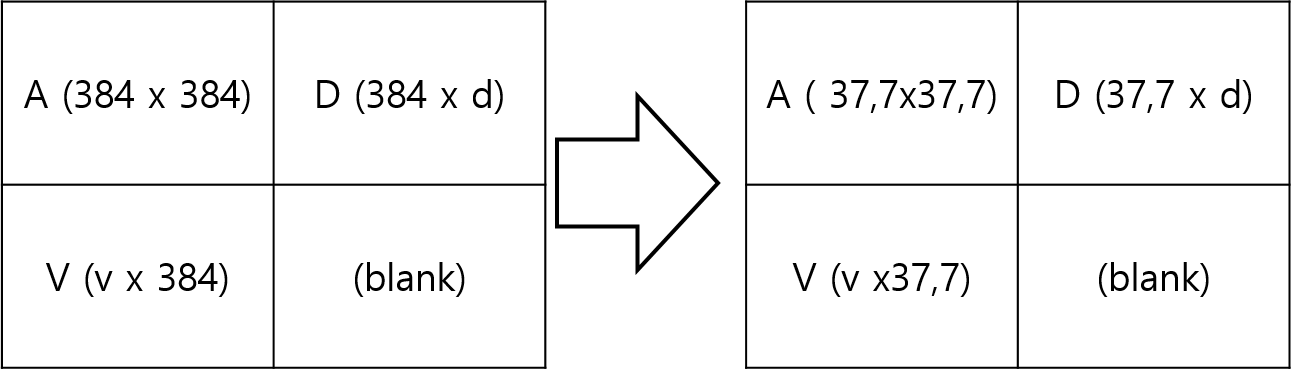
\includegraphics[width=1.00\textwidth]{IOagg.png}
	\end{figure}
		\begin{displaymath}
	\bar{a}_{I,J}=\sum_{i\in I}\sum_{j\in J} a_{i,j}\qquad\bar{v}_{v,J}=\sum_{j \in J}v_{v,j}\qquad\bar{d}_{I,d}=\sum_{i\in I}d_{i,d}
	\end{displaymath}
\end{frame}
%------------------------------------------------------------------------------	

%------------------------------------------------------------------------------
\begin{frame}[fragile]
	\frametitle{IO aggregation:agg\_1202.r}
\begin{scriptsize}
	\begin{verbatim}
## Step 1. Data preperation
#(i) loading
IOT_b=read.csv(file="IOT_b.csv",header=T, as.is=T)
sector_ind=read.csv(file="indcode_20161202.csv",header=T, as.is=T)

## Step 2. Rowsum:  merge and obtain rowsum using aggregate function
IOT_b_sec=merge(IOT_b,row_ind, by="basecode_row", all=T)
IOT_b_37=aggregate(IOT_b_sec[,4:(dim_IOT_b[2])],
list(IOT_b_sec$sector_row),FUN=sum)

## Step 3. Column sum
#(i) Traspose rowsum 
T_IOT_b_37=data.frame(t(IOT_b_37))
T_IOT_37_col=aggregate(T_IOT_b_37[,1:(nsector+nva)],
list(T_IOT_b_37$basecode_col),FUN=sum)

## Step 4. obtain IO table
#(i)obtain transpose of column sum
IOT_37=data.frame(t(T_IOT_37_col))
#(ii) add column names
colnames(IOT_37)[1:nsector]=sec_group[(1:37),2]
colnames(IOT_37)[(nsector+1):(nsector+nfd)]=fd_ind[,2]

write.csv(IOT_37, file="IO_model_1202.csv")
	\end{verbatim}
\end{scriptsize}	
\end{frame}
%-----------------------------------------------------------------
\section{ 3. SAM}

%------------------------------------------------------------------------------
\begin{frame}
	\frametitle{3. SAM :IO의 item을 이용해서 SAM 만들기}
	\begin{enumerate}
	\item{가계-정부 간 소득이전: 소득세, 이전지출}
	\item{부문 별 저축 확정}
		\begin{itemize}
		\item{가계저축 = 요소소득 + 이전소득 - 민간소비}
		\item{정부저축 = 조세수입 - 정부소비 - 이전지출}
		\item{해외저축 = 수입액 - 수출액 }
		\end{itemize}
	\end{enumerate}
	\begin{figure}
		\centering
		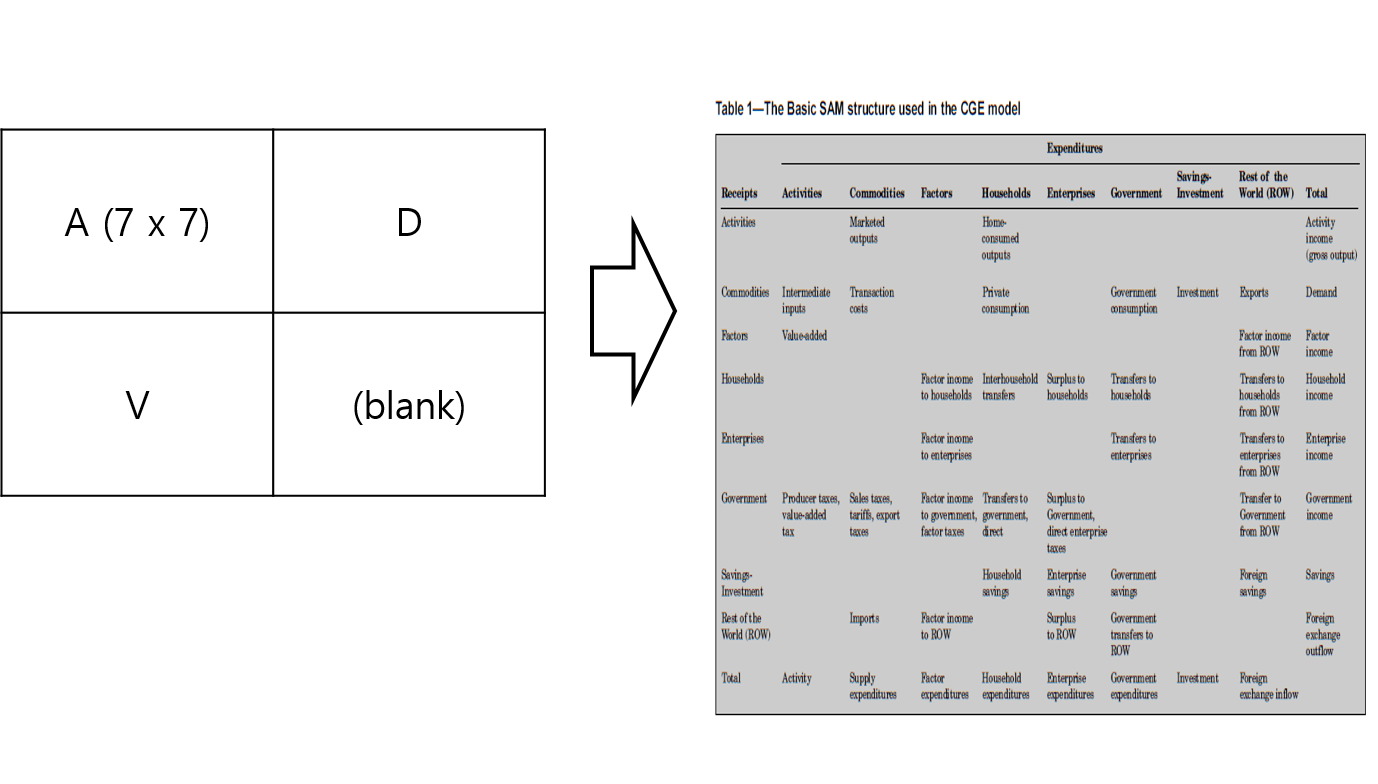
\includegraphics[width=1.00\textwidth]{IOtoSAM.png}
	\end{figure}


\end{frame}
%------------------------------------------------------------------------------


%------------------------------------------------------------------------------
\begin{frame}
	\frametitle{SAM}

	\begin{figure}
		\centering
		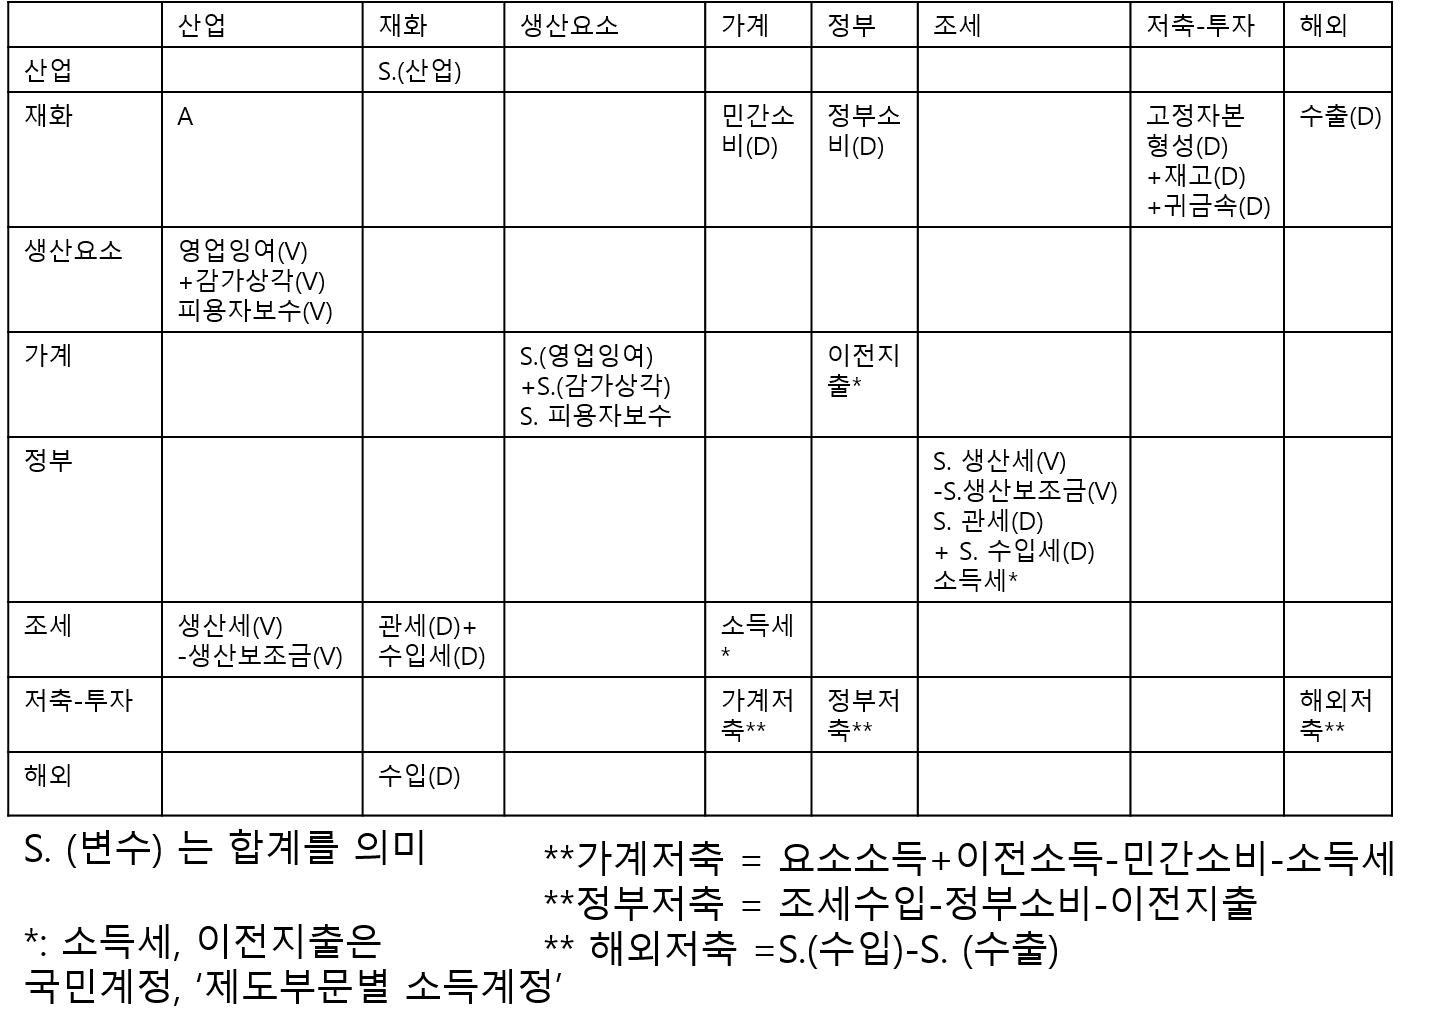
\includegraphics[width=1.00\textwidth]{sam.png}
	\end{figure}
\end{frame}
%------------------------------------------------------------------------------	

		
%------------------------------------------------------------------------------
\begin{frame}
	\frametitle{input-output}

		\begin{description}
			\item[input]
			\begin{enumerate}
			\item{Aggregated IO}
				\begin{itemize}
				\item{IO\_model\_1202.csv (37개 산업 IO)}
				\item{IO\_B\_1202.csv (7개 산업 IO)}
				\end{itemize}
			\item{Aggregated GHG IO}
				\begin{itemize}
				\item{GHG\_model\_p\_1202.csv (37개 산업 온실가스IO)}   
				\item{GHG\_BR\_p\_1202.csv (7개 산업 온실가스IO)}
				\end{itemize}
			\end{enumerate}
			\item[output]
				\begin{enumerate}
					\item{온실가스가 반영된 SAM} 
					\begin{itemize}
					\item{b\_sam\_36\_g\_pos\_1202.csv (37개산업)}
					\item{b\_sam\_br\_g\_1202.csv(7개산업)}
					\end{itemize}
					\item{온실가스가 반영되지 않은 SAM}
					\begin{itemize}
					\item{b\_sam\_36\_ng\_pos\_1202.csv(37개산업)}
					\item{b\_sam\_br\_ng\_1202.csv(7개산업)}
					\end{itemize} 
				\end{enumerate}
			\item[Process]
				\begin{enumerate}
					\item{samconst\_2010\_pos\_1202.r}				
				\end{enumerate}
					
		\end{description}
%	\end{enumerate}
\end{frame}
%------------------------------------------------------------------------------

%------------------------------------------------------------------------------
\begin{frame}[fragile]
	\frametitle{SAM 구축:samconst\_2010\_pos\_1202.r}
\begin{scriptsize}
	\begin{verbatim}
## load sam aggregation function
source("agg_1202.r")
source("agg_ghg_1202.r")
source("sam_2010.r")

#STEP 1: Size.SAM Determine the size of SAM   
ind=37;green=1;fac=2;h=1;gov=1;Nres=1;tax=4;S_I=1;ROW=1
Size.Sam=c(ind,green,fac,h,gov,Nres,tax,S_I,ROW)

#STEP 2: data.out : NON I-O data
YTAX=83753*1000
TRANSFER=39046*1000
data.out=c(YTAX,TRANSFER)

# STEP 3: I-O data ##load I-O data (model)
IO_model=read.csv("IO_model_1202.csv",header=T, as.is=T)
DIO=as.matrix(IO_model2)

#STEP 4: SAM construction
SAM_model=data.frame(SAM_agg_basic(Size.Sam,data.out,DIO))
model_SAM_name=c(m_Activity_name,"CO2-a",m_commodity_name,"CO2-c",
factor_name,Inst_name1,tax_name,Inst_name2)
rownames(SAM_model)=model_SAM_name
colnames(SAM_model)=model_SAM_name
		\end{verbatim}
\end{scriptsize}	
\end{frame}
%-----------------------------------------------------------------

%------------------------------------------------------------------------------
\begin{frame}
	\frametitle{b\_sam\_br\_g\_1202.csv}

	\begin{figure}
		\centering
		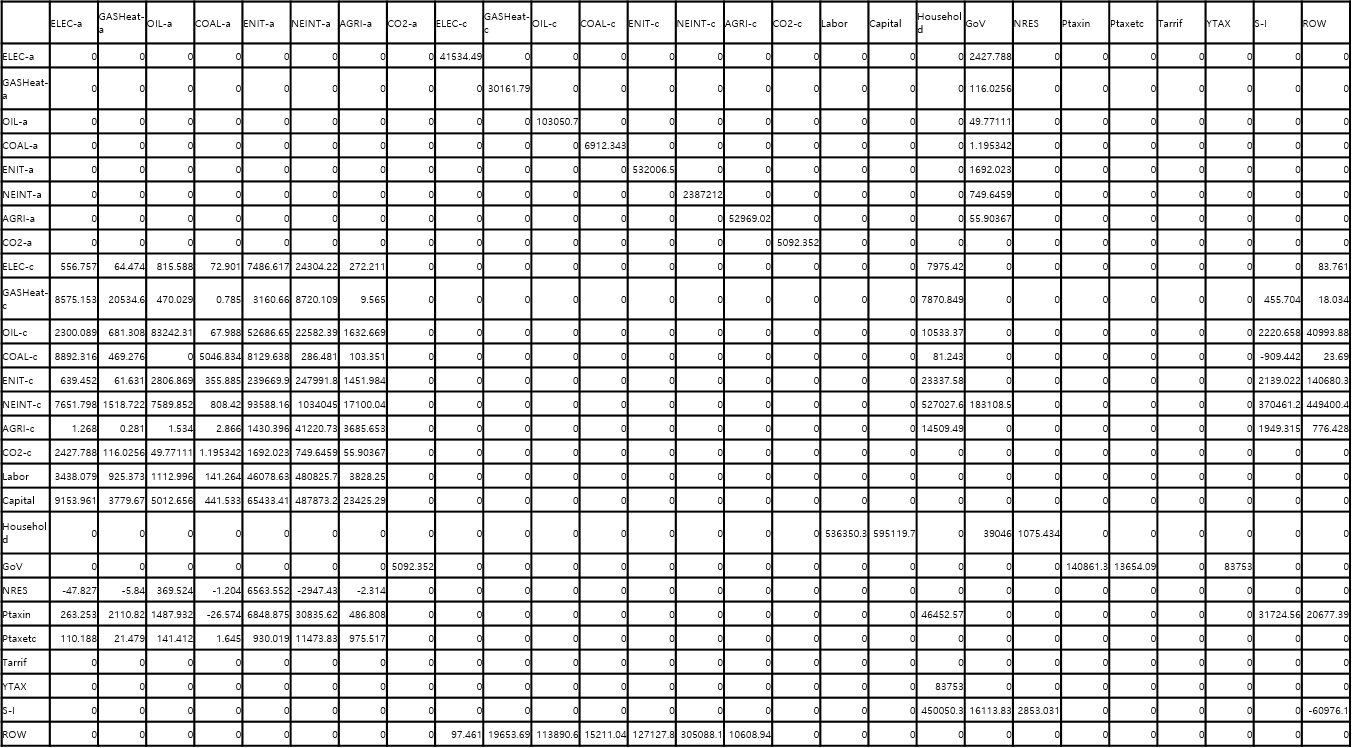
\includegraphics[width=1.00\textwidth]{samex.png}
	\end{figure}
\end{frame}
%------------------------------------------------------------------------------	

\section{4.Set}

%------------------------------------------------------------------------------
\begin{frame}
	\frametitle{4.set}
\begin{itemize}
\item{Contingent Set의 정의가 Data에 따라 변화$\rightarrow$ Contingent set이 활용된 program code는 Data 변화에 영향}
\bigskip
\item{*: Contingent Set의 변화에 따라 영향을 받을 수 있는 부분(Agritoy\_recursive.gms)}
\begin{small}
\begin{enumerate}
\item{Declaration (set)*}
\item{Data Loading*}
\item{Equations*}
\item{Calibration(Parameter,Initial value)*}
\item{Model Statement}
\item{Initialization}
\item{Solve Statement}
\item{Save and dispatch}
\end{enumerate}
\end{small}
\bigskip
\item{Agritoy\_recursive.gms의 경우 contingency set의 구성이 sector 변환 이전과 동일하여서 SAM과 CGE의 일관성이 유지}\end{itemize}
\end{frame}
%------------------------------------------------------------------------------

%------------------------------------------------------------------------------
\begin{frame}[fragile]
	\frametitle{Contingency Set}

Contingent Set: joint set 으로 한 집합의 element에 따라 다른 집합의 구성요소가 달라지는 set
\begin{scriptsize}
\begin{verbatim}
FD_C(C,FD)
/
GASHeat-c.(S-I )
OIL-c.(S-I )
COAL-c.(S-I )
ENIT-c.(S-I )
NEINT-c.(GoV,S-I )
Agri-c.(S-I )
/

ComMENCN(C)$(ENCN(C))..XA(C)=g=sum(A$XAPA(C,A),XAP(C,A))      
+sum(H$XACH(H,C),XAC(C,H))+sum(FD$FD_C(C,FD),XAF(FD,C));
\end{verbatim}
\end{scriptsize}
\end{frame}
%------------------------------------------------------------------------------

%------------------------------------------------------------------------------
\begin{frame}[fragile]
	\frametitle{Set Declaration의 자동화 (setwritting\_2015\_br\_1202.r)}

\begin{scriptsize}
\begin{verbatim}
sam_br=read.csv(file="b_sam_br_ng_1202.csv",header=T,as.is=T)
ghg=read.csv(file="GHG_BR_p_1202.csv",header=T,as.is=T)
filename="set_br_20151204.txt"
sink(file=filename)

#Non household (Domestic) Final demand: FD
FD=c("GoV","S-I")

#Final demand mix for non household institutions   
XFA=sam_br[Commodity,match(FD,colnames(sam_br))]
T_XFA=data.frame(t(XFA))
colnames(T_XFA)=rownames(XFA)
Positive.fin.demand=lapply(T_XFA,function(x){rownames(T_XFA)[x!=0]})
Positive.fin.demand=Positive.fin.demand[mapply(FUN=length,Positive.fin.demand)>0]
XFA.A={}
for (i in (1:length(Positive.fin.demand))){
  XFA.A_i=paste(paste(names(Positive.fin.demand)[i],HC.com(Positive.fin.demand[[i]]),sep=".("),")")
  XFA.A=rbind(XFA.A,XFA.A_i)
}
cat("FD_C(C,FD)",sep="\n")
cat("/",sep="\n")
cat(XFA.A,sep="\n")
cat("/",sep="\n")

\end{verbatim}
\end{scriptsize}
\end{frame}
%------------------------------------------------------------------------------

%------------------------------------------------------------------------------
\begin{frame}[fragile]
	\frametitle{Set Declaration의 자동화: output (set\_br\_20151211.txt)}

\begin{scriptsize}
\begin{verbatim}
....
XEPA(C,A)
/
GASHeat-c.(ELEC-a,GASHeat-a,OIL-a,COAL-a,ENIT-a,NEINT-a,Agri-a )
OIL-c.(ELEC-a,GASHeat-a,OIL-a,COAL-a,ENIT-a,NEINT-a,Agri-a )
COAL-c.(ELEC-a,GASHeat-a,COAL-a,ENIT-a,NEINT-a,Agri-a )
/
FD(ACT) /GoV,S-I /
FD_C(C,FD)
/
GASHeat-c.(S-I )
OIL-c.(S-I )
COAL-c.(S-I )
ENIT-c.(S-I )
NEINT-c.(GoV,S-I )
Agri-c.(S-I )
/
.....
Alias(GC,GCP);
Alias(ENC,ENCPP);
ACNT(ACT)=yes;
ACNT('Total')=no;
\end{verbatim}
\end{scriptsize}
\end{frame}
%------------------------------------------------------------------------------
%----------------------------------------------------------------------------------------------
\begin{frame}[fragile]
\frametitle{...}
\bigskip
\bigskip
\bigskip
\bigskip
\begin{Huge}
$\qquad$$\qquad$$\qquad$$\qquad$감사합니다.
\end{Huge}
\end{frame}
%----------------------------------------------------------------------------------------------

\end{document}
